% Source: graduate-coursework/Sp26/CSCE775/Project/proposal_asv_3/proposal3_asv.tex
% Description: Four water-body types with characteristic environmental conditions. The policy is conditioned on water-body type via a one-hot encoding in the state vector, enabling adaptation of motion and sensing strategies to domain-specific energy costs and hazard profiles.

\documentclass[border=4pt]{standalone}
\usepackage{amsmath,amssymb}
\usepackage{pgfplots}
\usepackage{tikz}
\usepackage{xcolor}
\pgfplotsset{compat=1.18}
\usetikzlibrary{positioning, arrows.meta, shapes.geometric, fit, calc, backgrounds, patterns, decorations.pathreplacing}

\definecolor{Garnet}{HTML}{73000A}
\definecolor{Atlantic}{HTML}{466A9F}
\definecolor{Congaree}{HTML}{1F414D}
\definecolor{Horseshoe}{HTML}{65780B}
\definecolor{Rose}{HTML}{CC2E40}
\definecolor{Honeycomb}{HTML}{A49137}
\definecolor{Black90}{HTML}{363636}
\definecolor{Black70}{HTML}{5C5C5C}
\definecolor{Black50}{HTML}{A2A2A2}
\definecolor{Black30}{HTML}{C7C7C7}
\definecolor{Black10}{HTML}{ECECEC}
\definecolor{WarmGrey}{HTML}{676156}


\begin{document}
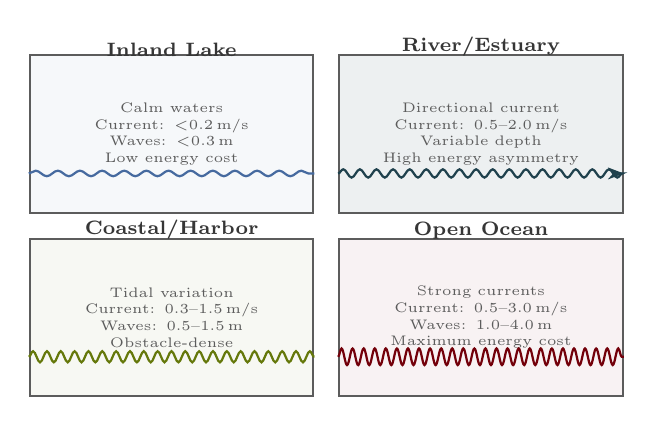
\begin{tikzpicture}[
    panel/.style={draw=Black70, thick, minimum width=3.6cm, minimum height=2.0cm, align=center},
    label/.style={font=\scriptsize\bfseries, color=Black90},
    desc/.style={font=\tiny, color=Black70, text width=3.2cm, align=center}
]

% Lake
\node[panel, fill=Atlantic!5] (lake) {};
\node[label, above=-0.15cm of lake.north] {Inland Lake};
\node[desc] at (lake.center) {Calm waters\\Current: $<$0.2\,m/s\\Waves: $<$0.3\,m\\Low energy cost};
\draw[thick, Atlantic, decorate, decoration={snake, amplitude=1pt, segment length=8pt}] ([yshift=-0.5cm]lake.west) -- ([yshift=-0.5cm]lake.east);

% River
\node[panel, fill=Congaree!8, right=0.3cm of lake] (river) {};
\node[label, above=-0.15cm of river.north] {River/Estuary};
\node[desc] at (river.center) {Directional current\\Current: 0.5--2.0\,m/s\\Variable depth\\High energy asymmetry};
\draw[thick, Congaree, -{Stealth[length=2mm]}, decorate, decoration={snake, amplitude=1.5pt, segment length=6pt}] ([yshift=-0.5cm]river.west) -- ([yshift=-0.5cm]river.east);

% Coastal
\node[panel, fill=Horseshoe!5, below=0.3cm of lake] (coast) {};
\node[label, above=-0.15cm of coast.north] {Coastal/Harbor};
\node[desc] at (coast.center) {Tidal variation\\Current: 0.3--1.5\,m/s\\Waves: 0.5--1.5\,m\\Obstacle-dense};
\draw[thick, Horseshoe, decorate, decoration={snake, amplitude=2pt, segment length=5pt}] ([yshift=-0.5cm]coast.west) -- ([yshift=-0.5cm]coast.east);

% Ocean
\node[panel, fill=Garnet!5, right=0.3cm of coast] (ocean) {};
\node[label, above=-0.15cm of ocean.north] {Open Ocean};
\node[desc] at (ocean.center) {Strong currents\\Current: 0.5--3.0\,m/s\\Waves: 1.0--4.0\,m\\Maximum energy cost};
\draw[thick, Garnet, decorate, decoration={snake, amplitude=3pt, segment length=4pt}] ([yshift=-0.5cm]ocean.west) -- ([yshift=-0.5cm]ocean.east);

\end{tikzpicture}
\end{document}
